\documentclass[11pt, a4paper]{article}
\usepackage{amsmath, amssymb, amsbsy}
\usepackage[amsmath, thmmarks]{ntheorem}
\usepackage{algorithm}
\usepackage{algpseudocode}
\usepackage{xcolor}
\usepackage{tikz}
\usepackage{paralist}
\usepackage{nicefrac}
\usepackage{minted}
% =========== 


% ============================= Pseudocode Customization =======================
% Packages: algorithm, algpseudocode.
\algrenewcommand{\algorithmicrequire}{\textbf{Input:}}
\algrenewcommand{\algorithmicensure}{\textbf{Output:}}
\algnewcommand\algorithmicto{\textbf{to} } % a trailing space is needed.
\algnewcommand\algorithmicbreak{\textbf{break}} % break keyword.
\newcommand{\breakif}[1]{\State \textbf{if} {#1} \textbf{then break}}


% ============================= Math Theorem Envs ==============================
\theorembodyfont{\normalfont}
\newtheorem{df}{Definition}[section]
\newtheorem{thm}[df]{Theorem}
\newtheorem{eg}[df]{Example}
\newtheorem{prop}[df]{Proposition}
\newtheorem{lem}[df]{Lemma}
\newtheorem{cor}[df]{Corollary}
\newtheorem{re}[df]{Remark}

% Customize proof env.
\theoremstyle{nonumberplain} % no numbering
\theoremsymbol{$\square$}    % proof end with square.
\newtheorem{pf}{Proof}


% =============================== Operators ====================================
\DeclareMathOperator{\ent}{Entropy}
\DeclareMathOperator*{\p}{\mathbb{P}} % probability.
\DeclareMathOperator{\sign}{sign}
\DeclareMathOperator*{\argmax}{argmax}
\DeclareMathOperator*{\argmin}{argmin}
\DeclareMathOperator*{\E}{\mathbb{E}} % Expectation.
\DeclareMathOperator{\dist}{dist} % distance.
\DeclareMathOperator{\indi}{\mathbb{I}}
\DeclareMathOperator{\tr}{tr} % trace of an matrix.


% =============================== New Commands =================================
% Logical connectives:
\newcommand{\OR}{\textbf{OR} } % a space is needed here.
\newcommand{\AND}{\textbf{AND} } 
\newcommand{\XOR}{\textbf{XOR} } 

% Math commands:
\newcommand{\T}[1]{\ensuremath{{#1}^\mathsf{T}}} % Matrix transposition.
\newcommand{\inv}[1]{\ensuremath{{#1}^{-1}}} % Inversion.
\newcommand{\V}[1]{\ensuremath{\boldsymbol{#1}}}

% Shorthand commands:
\newcommand{\hypo}[1]{\ensuremath{{#1}: \mathcal{X} \longrightarrow \mathcal{Y}}} % Hypothesis function.
\newcommand{\dataset}{\ensuremath{D = \{(\V{x}_1, y_1), \ldots, (\V{x}_m, y_m)\}}} % Labeled training set.
\newcommand{\st}{\text{s.t.\ }}
\newcommand{\magenta}[1]{\textcolor{magenta}{#1}} % turn the color of text into magenta.
\newcommand{\hl}[2][yellow]{\colorbox{#1}{#2}} % highlight the text.
\newcommand{\pfrac}[2]{\ensuremath{\frac{\partial {#1}}{\partial {#2}}}}

% =====================================================
\numberwithin{equation}{section}

% =============================Python Code Customization========================
% Package: minted
\setminted[python]{frame=single, linenos=true, numbersep=3pt, autogobble=true, mathescape=true}

% =============================== Document =====================================
\begin{document}

% ========Model Assessment and Selection======
\section{Model Assessment and Selection}


% ========Linear Models================
\section{Linear Models}
In a linear model, the learner takes the form of a (affine) linear function
$$y = \langle\V{w}, \V{x}\rangle + b = \langle\hat{\V{w}}, \hat{\V{x}}\rangle$$
where $\hat{\V{w}}=(\V{w}, b),\;\hat{\V{x}} = (\V{x}, 1)$.


% ========Decision Trees===============
\section{Decision Trees}
Decision Tree.

% ========SVM========================
\section{Support Vector Machine}

\subsection{Hard SVM}



\subsection{Soft SVM}

% ========Neuron Network
\section{Neuron Network}

% a 2 layer neuron network
\begin{figure}[h]
    \begin{center}
    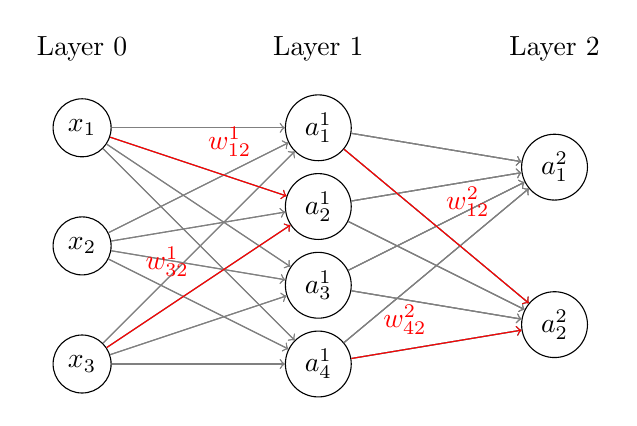
\begin{tikzpicture}
        % layer 0: input layer
        \begin{scope}[name prefix=layer0-]
            \node at (0, 0) {Layer 0};
            \node[circle, draw] (1) at (0, -1) {$x_1$};
            \node[circle, draw] (2) at (0, -2.5) {$x_2$};
            \node[circle, draw] (3) at (0, -4) {$x_3$};
        \end{scope}

        % layer 1
        \begin{scope}[name prefix=layer1-]
            \node at (3, 0) {Layer 1};
            \node[circle, draw] (1) at (3, -1) {$a^1_1$};
            \node[circle, draw] (2) at (3, -2) {$a^1_2$};
            \node[circle, draw] (3) at (3, -3) {$a^1_3$};
            \node[circle, draw] (4) at (3, -4) {$a^1_4$};
        \end{scope}

        % layer 2
        \begin{scope}[name prefix=layer2-]
            \node at (6, 0) {Layer 2};
            \node[circle, draw] (1) at (6, -1.5) {$a^2_1$};
            \node[circle, draw] (2) at (6, -3.5) {$a^2_2$};
        \end{scope}

        % weights
        \foreach \x in {1, 2, 3} {
            \foreach \y in {1, 2, 3, 4} {
                \foreach \z in {1, 2} {
                    \draw[gray, ->] (layer0-\x) -- (layer1-\y);
                    \draw[gray, ->] (layer1-\y) -- (layer2-\z);
                }
            }
        }
        \draw (layer0-1) edge[red, ->] node[auto] {$w^1_{12}$} (layer1-2);
        \draw (layer0-3) edge[red, ->] node[auto] {$w^1_{32}$} (layer1-2);
        \draw (layer1-1) edge[red, ->] node[auto] {$w^2_{12}$} (layer2-2);
        \draw (layer1-4) edge[red, ->] node[auto] {$w^2_{42}$} (layer2-2);
    \end{tikzpicture}
    \end{center}
    \caption{A 2 Layer Neuron Network}
\end{figure}

\subsection{Notations}
\begin{description}
    \item[$L$] output layer.
    \item[$n_l$] number of neurons in layer $l$. In particular, $n_0 = n$.
    \item[$w^l_{ij}$] weight from the $i$-th neuron in the layer $l-1$ to the $j$-th neuron in the layer $l$.
    \item[$b^l_j$] bias of the $j$-th neuron in layer $l$.
    \item[$a^l_j$] activation of the $j$-th neuron in layer $l$.
    \item[$z^l_j$] raw output of the $j$-th neuron in layer $l$.
    \item[$\sigma^l_j$] activation function of the $j$-th neuron in layer $l$.
    \item[$w^l$] weight matrix connecting layer $l-1$ to layer $l$, i.e. $(w^l_{ij})$, of dimension 
    $(n_{l-1},\ n_l)$.
    \item[$b^l$] bias vector of layer $l$, i.e. $(b^l_j)$, of dimension $(1, n_l)$.
    \item[$z^l$] raw output vector of layer $l$, of dimension $(1, n_l)$.
    \item[$a^l$] activation vector of layer $l$, of dimension $(1, n_l)$.
    \item[$\sigma^l$] activation function vector of layer $l$, of dimension $(1, n_l)$.
\end{description}

Some basic equations:

\begin{align}
    z^0_j &= a^0_j = x_j\\
    z^l_j &= \sum_k a^{l-1}_{k} w^l_{kj} + b^l_j\quad\forall~l\geq 1\\
    a^l_j &= \sigma^l_j(z^l_j)
\end{align}
The corresponding matrix forms are:

\begin{align}
    z^0 &= a^0 = \V{x} = (x_1, x_2, \ldots, x_{n})\\
    z^l &= a^{l-1} w^l + b^l\\
    a^l &= \sigma^l(z^l)
\end{align}

For a single input example \V{x}, the cost function $C$ should only directly depend on the output layer $L$,
for example $C$ is the square loss function:
\begin{equation}\label{nn_square_loss}
    C = \frac{1}{2} ||a^L - y||^2_2
\end{equation}
For a collection of examples, the cost function is the average cost on those examples:
\begin{equation}
    C = \frac{1}{m} \sum_{i=1}^m C(\V{x}_i)
\end{equation}

\subsection{Backpropagation}
Let $\delta^l_j$ be the error in the $j$-th neuron in the $l$-th layer, i.e.
\begin{equation}
    \delta^l_j = \pfrac{C}{z^l_j}
\end{equation}

For the output layer $L$, by definition we have:
\begin{align*}
    \delta^l_j &= \pfrac{C}{z^l_j}\\
               &= \sum_k \pfrac{C}{a^L_k} \pfrac{a^L_k}{z^L_j}\\
               &= \pfrac{C}{a^L_j} \pfrac{\sigma^L_j(z^L_j)}{z^L_j}\\
               &= \pfrac{C}{a^L_j} (\sigma^L_j)'(z^L_j)
\end{align*}
That is,
\begin{equation}
    \delta^L = \nabla_{a^L}C \odot (\sigma^L)'(z^L)
\end{equation}
When $C$ is the square loss~\eqref{nn_square_loss}, $\nabla_{a^L}C = a^L - y$.
\par
We can write $\delta^l$ in terms of $\delta^{l+1}$ as following:
\begin{align*}
    \delta^l_j &= \pfrac{C}{z^l_j}\\
               &= \sum_k \pfrac{C}{z^{l+1}_k} \pfrac{z^{l+1}_k}{z^l_j}\\
               &= \sum_k \delta^{l+1}_k \sum_r \pfrac{a^l_r}{z^l_j} w^{l+1}_{rk}\\
               &= \sum_k \delta^{l+1}_k (\sigma^l_j)'(z^l_j) w^{l+1}_{jk}\\
               &= {\left(\delta^{l+1} \T{(w^{l+1})}\right)}_{j} (\sigma^l_j)'(z^l_j)
\end{align*}
Its corresponding matrix form is:
\begin{equation}
    \delta^l = \left(\delta^{l+1} \T{(w^{l+1})}\right) \odot (\sigma^l)'(z^l)
\end{equation}

Now, let's compute \pfrac{C}{b^l_j}:
\begin{align*}
    \pfrac{C}{b^l_j} &= \sum_k \pfrac{C}{z^l_k} \pfrac{z^l_k}{b^l_j}\\
                     &= \sum_k \delta^l_k \pfrac{b^l_k}{b^l_j}\\
                     &= \delta^l_j
\end{align*}
In shorthand, it can be rewritten as:
\begin{equation}
    \pfrac{C}{b} = \delta
\end{equation}

Similarly, we can compute \pfrac{C}{w^l_{ij}}:
\begin{align*}
    \pfrac{C}{w^l_{ij}} &= \sum_k \pfrac{C}{z^l_k} \pfrac{z^l_k}{w^l_{ij}}\\
                        &= \sum_k \delta^l_k \sum_r \pfrac{(a^{l-1}_r w^l_{rk} + b^l_k)}{w^l_{ij}}\\
                        &= \sum_k \delta^l_k a^{l-1}_i \delta_{kj}\\
                        &= a^{l-1}_i \delta^l_j
\end{align*}
In shorthand, it can be rewritten as:
\begin{equation}
    \pfrac{C}{w} = a_{\text{in}}\delta_{\text{out}}
\end{equation}

For simplicity, let's assume that all the activation functions are the same, i.e. $\sigma^l_i = \sigma$, then 
we can write the pseudocode of backpropagation algorithm easily as the following:

\begin{algorithm}
    \caption{Backpropagation}\label{backpropagation}
    \begin{algorithmic}[1]
        \Require $\V{x} = (x_1, x_2, \ldots, x_n)$
        \For{$l = 1$ \algorithmicto $L$}
            \State Compute $z^l = a^{l-1} w^l + b^l$ and $a^l = \sigma(z^l)$.
        \EndFor
        \State Compute $\delta^l = \nabla_{a^L}C \odot \sigma'(z^L)$\Comment{$\nabla_{a^L}C = a^L - y$ if $C$ 
        is square loss.}
        \For{$l=L-1$ \algorithmicto $1$}
            \State Compute $\delta^l = \left(\delta^{l+1} \T{(w^{l+1})}\right) \odot \sigma'(z^l)$
        \EndFor
        \Ensure $\pfrac{C}{w^l_{ij}} = a^{l-1}_i \delta^l_j$ and $\pfrac{C}{b^l_j} = \delta^l_j$.
    \end{algorithmic}
\end{algorithm}

This is the algorithm for a single example, we are now ready to do the vectorization. Let $\V{x}^i$ and $y^i$
be the $i$-th example and its output respectively, let
\begin{align*}
    X &= {(\V{x}^1; \ldots; \V{x}^m)}_{m \times n}\\
    Y &= {(y^1; \ldots; y^m)}_{m \times n_L}
\end{align*}
the input matrix. 
Let $z^{i, l}, a^{i, l}, \delta^{i, l}$ be the raw output, output, error vectors w.r.t.\ the
$i$-th example respectively. Let 
\begin{align*}
    Z^l &= {(z^{1, l}; \ldots; z^{m, l})}_{m \times n_l}\\
    A^l &= {(a^{1, l}; \ldots; a^{m, l})}_{m \times n_l}\\
    \Delta^l &= {(\delta^{1, l}; \ldots; \delta^{m, l})}_{m \times n_l}
\end{align*}
then we have:
\begin{align}
    Z^l &= A^{l-1} w^l + b^l\\
    A^l &= \sigma(Z^l)\\
    \Delta^L &= \nabla_{A^L}C \odot \sigma'(Z^L)\\
    \Delta^l &= \left(\Delta^{l+1} \T{(w^{l+1})}\right) \odot \sigma'(Z^l)
\end{align}
If $C = \frac{1}{m}\sum_{i=1}^m C(\V{x}_i)$, then
$$\pfrac{C}{b^l_j} = \operatorname{reduce\_mean}(\operatorname{col}_j(\Delta^l))$$
and
$$\pfrac{C}{w^l_{ij}} = \operatorname{reduce\_mean}(\operatorname{col}_i(A^{l-1}) \odot \operatorname{col}_j
(\Delta^l))$$

% ========Bayesian Classifier=========
\include{sections/bayesian_classifier}

% ========Clustering=================
\include{sections/clustering}

% ========Expectation Maximalization====
\include{sections/EM}

% ========Ensemble Learning============
\section{Ensemble Learning}

\subsection{AdaBoost}

% AdaBoost algorithm
\begin{algorithm}
    \caption{AdaBoost}\label{AdaBoost}
    \begin{algorithmic}[1]
        \Require training set $D = \{(\V{x}_1, y_1), \ldots, (\V{x}_m, y_m)\}$; base learner $\mathcal{L}$;
        training round $T$.
        \State $\mathcal{D}_1(\V{x}) = \frac{1}{m}$.\Comment{$\mathcal{D}$ is a distribution over the input 
        examples.}
        \For{$t = 1$ \algorithmicto $T$}
            \State $h_t = \mathcal{L}(D, \mathcal{D}_t)$;
            \State $\varepsilon_t = \p_{\V{x}\sim\mathcal{D}_t}(h_t(\V{x})\neq f(\V{x}))$;\Comment{
            $\varepsilon_t$ is the error rate of $h_t$ w.r.t $\mathcal{D}_t$.}
            \State $\alpha_t = \frac{1}{2}\ln{\frac{1 - \varepsilon_t}{\varepsilon_t}}$;
            \State $\mathcal{D}_{t + 1}(\V{x}) = \frac{\mathcal{D}_t(\V{x})\exp(-\alpha_t f(\V{x})h_t(\V{x}))}
            {Z_t}$.\Comment{$Z_t$ is the normalization factor.}
        \EndFor
        \Ensure $H(\V{x}) = \sign(\displaystyle\sum_{t = 1}^T \alpha_t h_t(\V{x}))$
    \end{algorithmic}
\end{algorithm}

\subsection{Bagging}

% Bagging algorithm
\begin{algorithm}
    \caption{Bagging}\label{Bagging}
    \begin{algorithmic}[1]
        \Require training set $D = \{(\V{x}_1, y_1), \dotsc, (\V{x}_m, y_m)\}$; base learner $\mathcal{L}$;
        training round $T$.
        \For{$t = 1$ \algorithmicto $T$}
            \State $h_t = \mathcal{L}(D, \mathcal{D}_{bs})$\Comment{bs stands for bootstrap sampling.} 
        \EndFor
        \Ensure $H(\V{x}) = \displaystyle\argmax_{y\in \mathcal{Y}}\sum_{t=1}^T 1(h_t(\V{x}) = y)$\Comment{$H$
        is the plurality vote of $h_t$.}
    \end{algorithmic}
\end{algorithm}

\subsection{Random Forest}

% 

% ========Dimension Reduction=========
\section{Dimension Reduction}

\subsection{Low-dimensional embedding}
Let the feature space $\mathcal{X} = \mathbb{R}^d$. Our goal is to find an embedding of all samples into a
low dimension space $\mathbb{R}^{d'}$, here $d' \leq d$. That is, we want to find a map $e: \mathbb{R}^d
\longrightarrow \mathbb{R}^{d'}$ \st for any samples $\V{x}_i, \V{x}_j$, we have 
$$\dist(e(\V{x}_i), e(\V{x}_j)) = \dist(\V{x}_i, \V{x}_j)$$
Thus ${\left\{e(\V{x}_i)\right\}}_i$ is a low-dimensional embedding of the original samples. 

Let $\V{D} = {\left(\dist(\V{x}_i, \V{x}_j)\right)}_{m \times m}$ be the distance matrix of the samples 
${\left\{\V{x}_i\right\}}_i$, we want to find the embedding matrix $\V{Z} \in \mathbb{R}^{m \times d'}$, \st 
$||\V{z}_i - \V{z}_j|| = \V{D}_{ij}$, where $\V{Z} = (\V{z}_1; \dotsc; \V{z}_m)$ and 
$\V{D}_{ij} = \dist(\V{x}_i, \V{x}_j)$. Hence we have 
$$ \V{D}_{ij}^2 = ||\V{z}_i||^2 + ||\V{z}_j||^2 - 2 \langle\V{z}_i, \V{z}_j\rangle$$
Let $\V{B} = {\left(b_{ij}\right)}_{m \times m}= \V{Z}\T{\V{Z}}$ where $b_{ij} = \langle\V{z}_i, \V{z}_j\rangle$, 
we have
\begin{equation}\label{DR_Dij}
    \V{D}_{ij}^2 = b_{ii} + b_{jj} - 2 b_{ij}
\end{equation}
Let $\V{c} = \frac{1}{m}\sum_i \V{z}_i$, then ${\left\{\V{z}_i - \V{c}\right\}}_i$ is an embedding with the
property that $\sum_i(\V{z}_i - \V{c}) = 0$. Hence we can require that $\sum_i \V{z}_i = 0$ in the above
discussion. Then from equation~\eqref{DR_Dij}, we know that:
\begin{align}
    \sum_i \V{D}_{ij}^2 &= \tr(\V{B}) + m b_{jj}\\
    \sum_j \V{D}_{ij}^2 &= \tr(\V{B}) + m b_{ii}\\
    \sum_{i,j} \V{D}_{ij}^2 &= 2m \tr(\V{B})
\end{align}
From the above equations, we have
\begin{equation}\label{DR_bij}
    b_{ij} = -\frac{1}{2}\left(\V{D}_{ij}^2 - \frac{1}{m}\sum_i \V{D}_{ij}^2 - \frac{1}{m} \sum_j \V{D}_{ij}^2
    + \frac{1}{m^2}\sum_{i,j}\V{D}_{ij}^2\right)
\end{equation}
That is, $\V{B}$ is totally determined by $\V{D}$. Let $\V{B} = \V{V}\V{\Lambda}\T{\V{V}}$ be the eigenvalue
decomposition of $\V{B}$. Since $\V{B}$ is semi-positive, $\V{\Lambda}$ is a diagonal matrix with non-negative
diagonals. Let $\V{\Lambda}_*$ be the diagonal matrix obtained by removing the zero eigenvalues from 
$\V{\Lambda}$ and $\V{V}_*$ the matrix by removing the corresponding columns of $\V{V}$. Then it's easy to 
conclude that 
$$\V{Z} = \V{V}_*\V{\Lambda}_*^{\nicefrac{1}{2}}$$
is what we want. Hence the dimension $d'$ is totally determined by the distance matrix $\V{D}$. 

In practise, we often fix some $d' \ll d$ at first, then obtain $\V{\Lambda}_*$ by keeping the $d'$ largest 
eigenvalues and remove the rest, and $\V{V}_*$ the corresponding matrix. By this way, we may lose some 
precision in keeping the pairwise distance, but we can greatly reduce the dimension.

\begin{algorithm}
    \caption{Multiple Dimensional Scaling}
    \begin{algorithmic}[1]
        \Require the distance matrix $\V{D}_{m \times m}$; dimension $d'$.
        \State Compute the matrix $\V{B}$ according to equation~\eqref{DR_bij}.
        \State Eigenvalue decomposition: $\V{B} = \V{V} \V{\Lambda}\T{\V{V}}$.
        \State Let $\V{\Lambda}_*$ be the diagonal matrix with the $d'$ largest eigenvalues and $\V{V}_*$ the
        matrix with the corresponding eigenvectors.
        \Ensure Low-dimensional embedding: $\V{Z} = {\left(\V{V}_* \V{\Lambda}_*^{\nicefrac{1}{2}}\right)}_{m 
        \times d'}$
    \end{algorithmic}
\end{algorithm}

\subsection{Linear Dimension Reduction}
The simplest way to reduce dimension is by dropping some coordinates, that is, via projection. This keeps the
linear structure of the samples. A more generalized way is via linear transformation: $\V{X} \V{W} = \V{Z}$,
where $\V{X} = {\left(\V{x}_1; \dotsc; \V{x}_m\right)}_{m \times d}$ is the feature matrix of the samples, $\V{W} \in 
\mathbb{R}^{d \times d'}$ the transformation matrix, and $\V{Z}_{m \times d'}$ the representation matrix
in low dimensional space. If we write $\V{Z} = {\left(\V{z}_1; \dotsc; \V{z}_{m}\right)}$, then $\V{z}_i =
\V{x}_i \V{W}$.




% ========Computational Learning Theory
\section{Computational Learning Theory}
In this section, we mainly consider supervised learning.
Let $\mathcal{X}$ be the instance space, $\mathcal{Y}$ the label set, $D = \{(\V{x}_1, y_1), \ldots, 
(\V{x}_m, y_m)\}$ the training set. Assume $\mathcal{D}$ is the distribution on $\mathcal{X}$, and all 
instances of $D$ are sampled i.i.d.\ according to $\mathcal{D}$. Let \hypo{f} be the underlying labeling 
function and \hypo{h} any prediction function, then the \textbf{true (generalization) loss (error)} is defined
as:
$$L_{\mathcal{D}, f}(h) := \p_{\V{x}\sim\mathcal{X}}(h(\V{x})\neq f(\V{x})) := \mathcal{D}\left(\{\V{x}: h(\V{x})
\neq f(\V{x})\}\right)$$
the \textbf{empirical risk (error, loss)} is defined as:
$$L_S(h) = \frac{1}{m}\sum_{i=1}^m \indi(h(\V{x})\neq f(\V{x}))$$

\subsection{Probably Approximately Correct Learning}

% concept class.
\begin{df}[Concept class]
    A (target) concept is just a true labeling function \hypo{c}, that is, for any instace $(\V{x}, y)$ 
    (assuming sampling process is noise free) we have $c(\V{x}) = y$. The collection $\mathcal{C}$ of all 
    target concepts is called the concept class.
\end{df}

% hypothesis space.
\begin{df}[Hypothesis space]
    The collection of all labeling functions \hypo{f} a learner $\mathcal{L}$ can return is called the 
    hypothesis space (w.r.t.\ $\mathcal{L}$). We denote it as $\mathcal{H}$.
\end{df}

% inductive bias.
\begin{re}[Inductive bias]
    By restricting our learner to the hypothesis space instead of arbitrary predictors, we bias it toward a 
    particular set of predictors. Such restrictions are called \textbf{inductive bias}.
\end{re}

% realizability assumption.
\begin{df}[Realizability Assumption]
    The realizable assumption asserts that there is a $h^* \in \mathcal{H}$ s.t.\ 
    $L_{\mathcal{D}, f}(h^*) = 0$.
\end{df}

\begin{re}
    The realizable assumption implies that with probability 1 over i.i.d.\ samples $D$, we have $L_D(h^*) = 0$.
    That is, $\mathcal{D}^m(\{D: L_D(h^*) = 0\}) = 1$.
\end{re}

% PAC learnability.
\begin{df}[PAC learnability]\label{PAC_learnability}
    The concept class $\mathcal{C}$ is PAC learnable w.r.t.\ a hypothesis space $\mathcal{H}$ if there exist
    \begin{enumerate}
        \item a function $m: {(0, 1)}^2 \longrightarrow \mathbb{N}$;
        \item a learner $\mathcal{L}$.
    \end{enumerate}
    s.t.\ for any $\varepsilon, \delta \in (0, 1)$, for any distribution $\mathcal{D}$ over $\mathcal{X}$, and
    for any concept \hypo{c}, if the realizable assumption holds w.r.t.\ $\mathcal{H}, \mathcal{D}, c$, then
    when applying the learner $\mathcal{L}$ to $m \geq m(\varepsilon, \delta)$ i.i.d.\ samples generated by
    $\mathcal{D}$ and labeled by $c$, the learner returns a hypothesis $h$ s.t.\ with probability at least 
    $1 - \delta$ (over the choice of the samples), we have $L_{\mathcal{D},c}(h) \leq \varepsilon$. That is,
    $$\mathcal{D}^m(\{D: L_{\mathcal{D},c}(h) \leq \varepsilon\}) \geq 1 - \delta$$
\end{df}

% sample complexity.
\begin{df}[Sample complexity]
    The sample complexity of a learner is the minimal number of examples needed for the learner to produce a 
    PAC solution on any i.i.d.\ data sets with that many samples. That is, it is the minimum of all 
    $m(\varepsilon, \delta)$ where $m$ satisfies the requirements in definition~\ref{PAC_learnability}.
\end{df}

% agnostic PAC learnability.

% ========Reinforcement Learning
\section{Reinforcement Learning}

Let $X$ be the state space, $A$ the action space. Reinforcement learning can be described as a
\textbf{Markov Decision Process}: system changes from a state to another under the actions from $A$ with a 
rewarding function grading the change. That is, a reinforcement learning is a quadruple $E = \langle X, A, P,
R\rangle$, where $P: X \times A \times X \longrightarrow \mathbb{R}$ describes the probability of a state
changed into another via an action from $A$ and $R: X \times A \times X \longrightarrow \mathbb{R}$ describes
the reward of that change. Sometimes the rewarding function only depends on states, that is $R: X \times X
\longrightarrow \mathbb{R}$. Note that given a state $x$ and an action $a$ that can act on it, the resulting 
state $x'$ may not be unique, but the identity $\sum_{x'\in X}P_{x\rightarrow x'}^a = 1$ always holds true.
\par
The goal of reinforcement leanring is to find a \hl{policy $\pi$} dictating which action to take given a state
$x$. $\pi$ can be described in a determinate form $\pi: X \longrightarrow A$, which dictates that action
$\pi(x)$ must be performed on state $x$. It can also be described in a probability form: $\pi: X \times A
\longrightarrow \mathbb{R}$ where $\pi(x, a)$ is the probability of performing action $a$ on $x$. Obviously,
the determinate form is a special case of the probability form. The performance measurement of the policy is 
the accumulated reward gained from performing this policy for a reasonably long time. The \textbf{$T$ steps
accumulated reward} $\E[\frac{1}{T}\sum_{t=1}^{T}r_t]$ and \textbf{$\gamma$ discount accumulated reward}
$\E[\sum_{t=0}^{\infty}\gamma^t r_{t+1}]$ are two commonly used accumulated rewards, where $r_t$ is the reward
of step $t$.

\subsection{K-armed Bandit}
The K-armed bandit is a model of one step reinforcement learning. Every time you pull one arm of the machine,
it gives you some rewards with certain probability. The goal is to acquire as many rewards as possible.

\subsubsection{Exploration and Exploitation}
The \textbf{exploration-only} method tries to figure out the expectation reward of each arm. It divides the 
exploration chance evenly on each arm, and use the average reward of each arm as the expectation reward. This
method may do a good job in estimating each arm's reward, but it may miss the opportunity to get the most 
rewards. The \textbf{exploitation-only} method, on the other hand, only pulls the arm that gives the most 
average rewards so far. Since it dosen't care about the expectation reward of each arm, it may also miss the
opportunity to get the most rewards. 

\subsubsection{$\varepsilon$-greedy}
The $\varepsilon$-greedy is a compromise between exploration-only and exploitation-only method. At
each try, it performs exploration-only method with a probability $\varepsilon$ and exploitation-only method
the other $1 - \varepsilon$.\par
Let $Q_n(k)$ denote the average reward of arm $k$ with $n$ tries and $v_n^k$ its n-th reward, then it is 
clearly that
$$Q_n(k) = \frac{1}{n} ((n-1)Q_{n-1}(k) + v_n^k)$$
This is the updating rules for the average reward.

% epsilon-greedy algorithm
\begin{algorithm}
    \caption{$\varepsilon$-greedy}\label{epsilon_greedy_for_K_arm_bandit}
    \begin{algorithmic}[1]
        \Require number of arms $K$; rewarding function $R$; number of tries $T$; exploration threshold 
        $\varepsilon$.
        \State $r = 0$\Comment{the accumulated reward.}
        \State $Q(i) = 0, \quad count(i) = 0 \quad \forall~i=1,\ldots,K$\Comment{Initialization.}
        \For{$t = 1$ \algorithmicto $T$}
            \If{$rand() < \varepsilon$}
                \State $k = rand(\{1, \ldots, K\})$\Comment{choose with equal probability}
            \Else
                \State $k = \argmax_i Q(i)$
            \EndIf
            \State $v = R(k)$
            \State $r \gets r + v$
            \State $Q(k) \gets \frac{count(k) \cdot Q(k) + v}{count(k) + 1}$
            \State $count(k) \gets count(k) + 1$
        \EndFor
        \Ensure the accumulated reward $r$.
    \end{algorithmic}
\end{algorithm}

% TODO: analysis of the epsilon-greedy.

\subsubsection{Softmax}
Softmax algorithm is another way of compromising between the exploration-only and exploitation-only methods. 
Unlike the $\varepsilon$-greedy algorithm which uses a threshold to determine how to choose an arm, softmax 
attach each arm with a probability to be chosen base on its current average reward. The probability 
distribution among the arms is a Boltzmann distribution, namely:
\begin{equation}\label{K_arm_bandit_softmax}
P(k) = \frac{e^{\frac{Q(k)}{\tau}}}{\sum_{i=1}^K e^{\frac{Q(i)}{\tau}}}\quad\forall~k = 1,\ldots,K
\end{equation}
where the parameter $\tau > 0$. Apparently, if $\tau$ is close to $0$, the softmax favours the arm with
the highest average reward, which is the case of exploitation-only method; if $\tau$ is very large (close to 
$+\infty$), the softmax degenerates to uniform distribution, which is the case of exploration-only method.

% softmax algorithm for K-arm bandit.
\begin{algorithm}
    \caption{Softmax}\label{Softmax_for_K_arm_bandit}
    \begin{algorithmic}[1]
        \Require number of arms $K$; rewarding function $R$; number of tries $T$; parameter $\tau$.
        \State $r = 0$
        \State $Q(i) = 0, \quad count(i) = 0\quad\forall~i=1,\ldots, K$
        \For{$t = 1$ \algorithmicto $T$}
            \State choose $k$ according to the distribution given by equation~\eqref{K_arm_bandit_softmax}.
            \State $v = R(k)$
            \State $r \gets r + v$
            \State $Q(k) \gets \frac{count(k)\cdot Q(k)}{count(k) + 1}$
            \State $count(k) \gets count(k) + 1$
        \EndFor
        \Ensure the accumulated reward $r$.
    \end{algorithmic}
\end{algorithm}

% TODO: analysis of the softmax algorithm.

\newpage
\subsection{Model-based Learning}
In model-based learning, the quadruple $E = \langle X, A, P, R\rangle$ are known to us. That is, we know all
the possible states, all the possible actions that may act on them, the transition function which describes
the probability of one state changing into another under some action, the rewarding function which grades the
change. In the following discussion, we assume that \magenta{the state space $X$ and the action space $A$ are
finite}.

\subsubsection{Policy Measurement}
Let $V^\pi(x)$ be the expected reward gained from applying policy $\pi$ on the starting state $x$, 
$Q^\pi(x, a)$ the expected reward gained from first applying action $a$ then policy $\pi$ on the starting
state $x$. $V$ and $Q$ are called \textbf{state value function} and \textbf{state-action value function}
respectively. \par
By definition, we can write the state value function as:
\begin{align}
    V^\pi_T(x) &= \E_\pi\left[\frac{1}{T}\sum_{t=1}^{T}r_t | x_0 = x\right], &\text{$T$ steps}
    \label{state_value_T}\\
    V^\pi_\gamma(x) &= \E_\pi\left[\sum_{t=0}^{\infty} \gamma^t r_{t+1} | x_0 = x\right], &\text{$\gamma$ 
    discount}\label{state_value_gamma}
\end{align}
Similarly, we can write the state-action value function as:
\begin{align}
    Q^\pi_T(x, a) &= \E_\pi\left[\frac{1}{T}\sum_{t=1}^T r_t | x_0 = x, a_0 = a\right], &\text{$T$ steps}
    \label{state-action_value_T}\\
    Q^\pi_\gamma(x, a) &= \E_\pi\left[\sum_{t=0}^\infty \gamma^t r_{t+1} | x_0 = x, a_0 = a\right] &\text{
    $\gamma$ discount}\label{state-action_value_gamma}
\end{align}
Since the next state of the system only depends on the current state, those value functions can be written in
a recursive form. For example, the $T$ steps accumulated state value function~\eqref{state_value_T} can be 
written as:
\begin{align}
    V^\pi_T(x) &= \E_\pi \left[\frac{1}{T}\sum_{t=1}^T r_t | x_0 = x\right]\nonumber\\
               &= \E_\pi \left[\frac{1}{T} r_1 + \frac{T-1}{T}\frac{1}{T-1}\sum_{t=2}^T r_t | x_0 = x\right]
               \nonumber\\
               &= \sum_{a\in A}\pi(x, a)\sum_{x'\in X}P_{x\rightarrow x'}^a\left(\frac{1}{T}
               R_{x\rightarrow x'}^a + \frac{T-1}{T}\E_\pi\left[\frac{1}{T-1}\sum_{t=1}^{T-1}r_t | x_0=x'
               \right]\right)\nonumber\\
               &= \sum_{a\in A}\pi(x, a)\sum_{x'\in X}P_{x\rightarrow x'}^a\left(\frac{1}{T}
               R_{x\rightarrow x'}^a + \frac{T-1}{T} V^\pi_{T-1}(x')\right)
\end{align}
Similarly, the $\gamma$ discount accumulated state value function~\eqref{state_value_gamma} can be written as:
\begin{align}
    V^\pi_\gamma(x) &= \E_\pi\left[\sum_{t=0}^\infty \gamma^t r_{t+1} | x_0 = x\right]\nonumber\\
                    &= \E_\pi\left[r_0 + \gamma \sum_{t=1}^\infty \gamma^{t-1}r_{t+1} | x_0=x\right]\nonumber\\
                    &= \sum_{a\in A}\pi(x, a)\sum_{x'\in X}P_{x\rightarrow x'}^a \left(R_{x\rightarrow x'}^a + 
                    \gamma \E_\pi\left[\sum_{t=0}^\infty \gamma^t r_{t+1} | x_0 = x'\right]\right)\nonumber\\
                    &= \sum_{a\in A}\pi(x, a)\sum_{x'\in X}P_{x\rightarrow x'}^a \left(R_{x\rightarrow x'}^a +
                    \gamma V^\pi_\gamma(x')\right)
\end{align}

% algorithm for calculating T steps accumulated state value function.
\begin{algorithm}
    \caption{$T$ steps accumulated state value function}
    \begin{algorithmic}[1]
        \Require $E = \langle X, A, P, R\rangle$; policy $\pi$; steps $T$.
        \State $V(x) = 0\quad\forall~x\in X$
        \For{$t=1$ \algorithmicto $T$}
            \State $\displaystyle V'(x) = \sum_{a\in A}\pi(x,a)\sum_{x'\in X}P_{x\rightarrow x'}^a 
            \left(\frac{1}{t} R_{x\rightarrow x'}^a + \frac{t-1}{t}V(x')\right)\quad\forall~x\in X$
            \If{$t = T+1$}
                \State \algorithmicbreak
            \Else
                \State $V \gets V'$
            \EndIf
        \EndFor
        \Ensure state value function $V$.
    \end{algorithmic}
\end{algorithm}

% algorithm for gamma discount accumulated state value function.
\begin{algorithm}
    \caption{$\gamma$ discount accumulated state value function}
    \begin{algorithmic}[1]
        \Require $E = \langle X, A, P, R\rangle$; policy $\pi$; parameter $\gamma$; threshold $\theta$.
        \State $V(x) = 0\quad\forall~x\in X$
        \Loop
            \State $\displaystyle V'(x) = \sum_{a\in A}\pi(x,a)\sum_{x'\in X}P_{x\rightarrow x'}^a 
            \left(R_{x\rightarrow x'}^a + \gamma V(x')\right)\quad\forall~x\in X$
            \If{$\displaystyle\max_{x\in X}|V(x) - V'(x)| < \theta$}
                \State \algorithmicbreak
            \Else
                \State $V \gets V'$
            \EndIf
        \EndLoop
        \Ensure state value function $V$.
    \end{algorithmic}
\end{algorithm}

% TODO: formulas for state-action value functions.

% TODO: algorithms for state-action value functions.

\subsubsection{Policy Improvement}

\subsection{Model-free Learning}


\end{document}